% !TeX TXS-program:compile = txs:///arara
% arara: lualatex: {shell: no, synctex: yes, interaction: batchmode}
% arara: pythontex: {rerun: modified} if exists('pytxcode') && found('pytxcode', 'PYTHONTEX#py')
% arara: lualatex: {shell: no, synctex: yes, interaction: batchmode} if exists('pytxcode') && found('pytxcode', 'PYTHONTEX#py')
% arara: lualatex: {shell: no, synctex: yes, interaction: batchmode} if found('log', '(undefined references|Please rerun|Rerun to get)')

\documentclass[a4paper,11pt]{article}
\usepackage[revgoku]{cp-base}
\graphicspath{{./graphics/}}
%variables
\donnees[classe={1\up{ère} 2M2},matiere={[SPÉ.MATHS]},mois=Mai,annee=2022,typedoc=CHAP,numdoc=11]

%formatage
\author{Pierquet}
\title{\nomfichier}
\hypersetup{pdfauthor={Pierquet},pdftitle={\nomfichier},allbordercolors=white,pdfborder=0 0 0,pdfstartview=FitH}
%divers
\lhead{\entete{\matiere}}
\chead{\entete{\lycee}}
\rhead{\entete{\classe{} - \mois{} \annee}}
\lfoot{\pied{\matiere}}
\cfoot{\logolycee{}}
\rfoot{\pied{\numeropagetot}}

\begin{document}

\pagestyle{fancy}

\part{CH11 - Applications de la dérivation - Exercices}

\medskip

\begin{caide}
	{\setlength\arrayrulewidth{1.5pt} \arrayrulecolor{titrebleu!35}
		\begin{tabularx}{\linewidth}{Y|Y|Y|Y|Y|Y}
			\niveaudif{0}~~\textsf{Basique} & \niveaudif{1}~~\textsf{Modérée} & \niveaudif{2}~~\textsf{Élevée} & \niveaudif{3}~~\textsf{Très élevée} & \niveaudif{4}~~\textsf{Extrême} & \niveaudif{5}~~\textsf{Insensée} \\
	\end{tabularx}}
\end{caide}

\exonum{0}

\medskip

Soit $g$ une fonction définie et dérivable sur l'intervalle $I=\intervFO{0}{+\infty}$. Le tableau suivant donne le signe de $g'(x)$ sur $I$.
\begin{center}
	\begin{tikzpicture}
		\tkzTabInit{$x$/0.6,$g'(x)$/0.6}{$0$,$3$,$6$,$+\infty$}
		\tkzTabLine{,-,z,+,z,-,}
	\end{tikzpicture}
\end{center}
\begin{enumerate}
	\item Sachant que $g(3)=-1$ et $g(6)=2$, dresser le tableau de variations de $g$.
	\item Tracer une courbe susceptible de représenter la fonction $g$.
\end{enumerate}

\medskip

\exonum{1}

\medskip

La courbe $\mathscr{C}$ ci-dessous représente une fonction $k$ définie et dérivable sur $\intervFF{-8}{6}$.
%
\begin{center}
	\tunits{0.45}{0.45}
	\tdefgrille{-9}{7}{1}{1}{-2}{8}{1}{1}
	\begin{tikzpicture}[x=\xunit cm,y=\yunit cm]
		%grilles & axes
		\tgrilles[line width=0.3pt,lightgray!50] ;
		\tgrillep[line width=0.6pt,lightgray!50] ;
		\axestikz*[width=0.75pt] ;
		\foreach \x in {-9,-8,...,6} \draw[line width=0.75pt] (\x,-3pt) -- (\x,3pt) ;
		\foreach \y in {-2,-1,...,7} \draw[line width=0.75pt] (-3pt,\y) -- (3pt,\y) ;
		\foreach \x in {-5,1,5} \draw (\x,-3pt) node[below] {\footnotesize $\num{\x}$} ;
		\foreach \y in {1,5} \draw (-3pt,\y) node[left] {\footnotesize $\num{\y}$} ;
		\draw (-1pt,-1pt) node[below left] {\footnotesize $0$} ;
		\draw[red] (6,5) node {$\mathscr{C}$} ;
		%\axextikz[width=0.75pt,size=\footnotesize]{-9,-8,...,6} ;
		%\axeytikz[width=0.75pt,size=\footnotesize]{-2,-1,...,7} ;
		\clip (\xmin,\ymin) rectangle (\xmax,\ymax) ; %on restreint les fonctions à la fenêtre
%		%les splines en pgf
%		\draw[line width=1.25pt,red,samples=200,domain=-8:-5] plot(\x,{-0.0741*\x*\x*\x+-1.4444*\x*\x+-8.8889*\x+-16.5926}) ;
%		\draw[line width=1.25pt,red,samples=200,domain=-5:-4] plot(\x,{4.0*\x*\x*\x+54.0*\x*\x+240.0*\x+351.0}) ;
%		\draw[line width=1.25pt,red,samples=200,domain=-4:0] plot(\x,{-0.1562*\x*\x*\x+-0.9375*\x*\x+0.0*\x+4.0}) ;
%		\draw[line width=1.25pt,red,samples=200,domain=0:3] plot(\x,{0.2963*\x*\x*\x+-1.3333*\x*\x+0.0*\x+4.0}) ;
%		\draw[line width=1.25pt,red,samples=200,domain=3:6] plot(\x,{-0.1852*\x*\x*\x+3.0*\x*\x+-13.0*\x+17.0}) ;
		%splinetikz
		\def\LISTE{-8/0/0§-5/1/0§-4/-1/0§0/4/0§3/0/0§6/7/3}
		\splinetikz[liste=\LISTE,couleur=red,,coeffs=3§2§3§3§2]
		%points de contôle
		\foreach \Point in {(-8,0),(-5,1),(-4,-1),(0,4),(3,0),(6,7)} \filldraw[red] \Point circle[radius=2pt] ;
	\end{tikzpicture}
\end{center}
%
\begin{enumerate}
	\item Quel est le maximum local de $k$ sur $\intervFF{-8}{-4}$ ?
	\item Quel est le minimum local de $k$ sur $\intervFF{-8}{0}$ ?
	\item Quel est le maximum de $k$ sur $\intervFF{-8}{6}$ ?
	\item Quel est le minimum de $k$ au voisinage de $3$ ?
\end{enumerate}

\exonum{1}

\medskip

Soit $f$ la fonction définie et dérivable sur $\R$ par $f(x)=-x^3+x^2+x+2$.
\begin{enumerate}
	\item Déterminer $f'(x)$.
	\item Étudier le signe de $f'(x)$ sur $\R$ puis en déduire le tableau de variations de $f$ sur $\R$.
\end{enumerate}

\medskip

\exonum{2}

\medskip

On considère la fonction $h$ définie par $h(x)=\dfrac{-x^2+8x-13}{x^2-4x+5}$.
\begin{enumerate}
	\item Justifier que $h$ est définie sur $\R$, puis vérifier que, pour tout réel $x$, on a $h'(x)=\dfrac{-4x^2+16x-12}{\big( x^2-4x+5\big)^2}$.
	\item Étudier le signe de $h'(x)$ puis dresser le tableau de variations de $h$ sur $\R$.
\end{enumerate}

\medskip

\exonum{2}

\medskip

On considère la fonction $f$ définie (et dérivable) sur $I=\intervFF{1}{6}$ par $f(x)=2x-10+\dfrac{8}{x}$.
\begin{enumerate}
	\item Déterminer $f'(x)$.
	\item Étudier le signe de $f(x)$ puis dresser le tableau de variations complet de $f$ sur $I$.
	\item En déduire l'existence d'un minimum pour $f$ sur $I$. Préciser sa valeur et la valeur de $x$ pour lequel il est atteint. 
	\item On donne $f(4)=0$. Déterminer le tableau de signes de $f(x)$ sur $I$.
	\item Déterminer, en justifiant, le nombre de solutions de $f(x)=-1$.
\end{enumerate} 

\medskip

\exonum{2}

\medskip

On donne ci-dessous le courbe représentative d'une fonction $f$, définie et dérivable sur $\R$, dans un repère orthonormé.
\begin{center}
	\tunits{1}{1}
	\tdefgrille{-2.25}{3.25}{1}{1}{-1.25}{3.25}{1}{1}
	\begin{tikzpicture}
		\tgrilles[color=cyan,line width=0.4pt] ;
		\axestikz* ;
		\axextikz{-2,-1,...,3} ; \axeytikz{-1,0,...,3} ;
		\clip (\xmin,\ymin) rectangle (\xmax,\ymax) ;
		\draw[line width=1.25pt,red,domain=\xmin:\xmax,samples=200] plot (\x,{-1/4*\x*\x*\x*\x + 1/3 * \x*\x*\x+\x*\x+1/3}) ;
		\draw[line width=1.25pt,darkgray,<->] (1,3) -- (3,3) ;
		\draw[line width=1.25pt,darkgray,<->] (-2,0.75) -- (0,0.75) ;
		\draw[line width=1.25pt,darkgray,<->] (-1,{1/3}) -- (1,{1/3}) ;
	\end{tikzpicture}
\end{center}
%
\begin{enumerate}
	\item Déterminer le tableau de variations de $f$ puis en déduire le tableau de signes de $f'(x)$.
	\item L'une des trois courbes ci-dessous représente graphiquement la fonction $f'$. Laquelle ?
\end{enumerate}
\begin{center}
	\tunits{1}{1}
	\tdefgrille{-2.25}{3.25}{1}{1}{-3.25}{1.25}{1}{1}
	\begin{tikzpicture}
		\tgrilles[color=cyan,line width=0.4pt] ;
		\axestikz* ;
		\axextikz{-2,-1,...,3} ; \axeytikz{-3,-2,...,1} ;
		\clip (\xmin,\ymin) rectangle (\xmax,\ymax) ;
		\draw[line width=1.25pt,orange,domain=\xmin:\xmax,samples=200] plot (\x,{0.5*\x*(\x+1)*(\x+1)*(\x-2)}) ;
		\draw[orange] (-2,0.75) node[below right=0pt,font=\large] {$\mathscr{C}_1$} ;
	\end{tikzpicture}
	\hspace{0.25cm}
	\tdefgrille{-2.25}{3.25}{1}{1}{-2.25}{2.25}{1}{1}
	\begin{tikzpicture}
		\tgrilles[color=cyan,line width=0.4pt] ;
		\axestikz* ;
		\axextikz{-2,-1,...,3} ; \axeytikz{-2,-1,...,2} ;
		\clip (\xmin,\ymin) rectangle (\xmax,\ymax) ;
		\draw[line width=1.25pt,blue,domain=\xmin:\xmax,samples=200] plot (\x,{-1/3*(\x+1)*(\x-2)*(\x-2)}) ;
		\draw[blue] (-2,2) node[below right=0pt,font=\large] {$\mathscr{C}_2$} ;
	\end{tikzpicture}
	\hspace{0.25cm}
	\tdefgrille{-2.25}{3.25}{1}{1}{-1.75}{2.75}{1}{1}
	\begin{tikzpicture}
		\tgrilles[color=cyan,line width=0.4pt] ;
		\axestikz* ;
		\axextikz{-2,-1,...,3} ; \axeytikz{-1,0,...,2} ;
		\clip (\xmin,\ymin) rectangle (\xmax,\ymax) ;
		\draw[line width=1.25pt,ForestGreen,domain=\xmin:\xmax,samples=200] plot (\x,{-\x*\x*\x+\x*\x+2*\x}) ;
		\draw[ForestGreen] (-2,2) node[above right=0pt,font=\large] {$\mathscr{C}_3$} ;
	\end{tikzpicture}
\end{center}

\medskip

\exonum{3}

\medskip

Soit $f$ la fonction définie et (deux fois) dérivable sur $\R$ par $f'(x)=3x^4-4x^3+6x^2-12x+12$.
%
\begin{enumerate}
	\item Calculer $f'(x)$ puis $f''(x)$ (dérivée de $f'$).
	\item
	\begin{enumerate}
		\item Étudier le signe de $f''(x)$.
		\item En déduire le tableau de variation de $f'$ sur $\R$.
	\end{enumerate}
	\item 
	\begin{enumerate}
		\item Calculer $f'(1)$ puis en déduire le signe de $f'(x)$ sur $\R$.
		\item Dresser finalement le tableau de variations de $f$ sur $\R$.
	\end{enumerate}
\end{enumerate}

\end{document}